\begin{chapter}{Der Beweis von Robertson, Sanders, Seymour und Thomas}
  Die Grundidee des Beweises besteht darin, eine bestimmte Menge von 633 sogenannten Konfigurationen -- welche nicht mit den Konfigurationen von Appel \& Haken zu verwechseln sind -- aufzustellen und dann zu zeigen, dass kein Element dieser Menge in einem minimalen Gegenbeispiel vorkommen kann -- dieser erste Schritt wird \textit{Reduzierbarkeit} (engl.: reducibility) genannt. Damit folgt der Beweis der Idee seiner Vorgänger, allerdings mit dem Unterschied, dass jedes minimale Gegenbeispiel eine \textit{intern 6-fach zusammenhängende Triangulation} ist. \\
  Im zweiten Schritt wird gezeigt, dass in jeder intern 6-fach zusammenhängenden Triangulation eine der oben genannten Konfigurationen vorkommen muss -- auch \textit{Zwangsläufigkeit} (eng.: unavoidability) genannt. Zusammen zeigt dies, dass es kein minimales Gegenbeispiel geben kann und der Vierfarbensatz somit wahr ist. \\
  Der wesentliche Unterschied zum vorher vorgestellten Beweis von Appel \& Haken liegt darin, auf welche Art die Zwangsläufigkeit hergestellt wird.
  
    \begin{section}{Die Konfigurationen}
   Eine Klasse von Graphen ist für den Beweis des Vier-Farben-Satzes wesentlich: Die Konfigurationen. Sie treten vor allem als Untergraphen der normalen Graphen auf. Zuerst wollen wir festhalten, was eine Konfiguration eigentlich ist.
   
   \begin{definitionl}{Konfiguration}{konfig}
    Ein Graph $C$ heißt \textit{Konfiguration}, wenn
    \begin{itemize}
     \item er regulär ist,
     \item die Außenecken einen Ring der Größe größer-gleich 4 bilden,
     \item innere Ecken existieren,
     \item die beschränkten Gebiete von Dreiecken begrenzt werden,
     \item jedes Dreieck Grenze eines Gebiets ist.
    \end{itemize}
   \end{definitionl}
   
   Ein nicht-triviales Beispiel für eine Konfiguration ist der \textit{Birkhoff}-Diamant.
   
    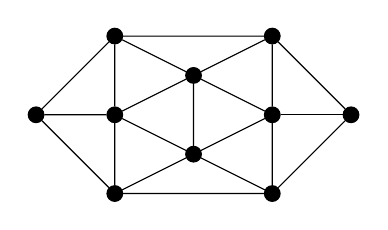
\begin{tikzpicture}[every node/.style={draw,inner sep=2pt,fill=black}]
      \path[shape=circle]
	(0,1) node(a1){} 
	(1,0) node(b1){} (1,1) node(b2){} (1,2) node(b3){}
	(2,0.5) node(c1){} (2,1.5) node(c2){}
	(3,0) node(d1){} (3,1) node(d2){} (3,2) node(d3){}
	(4,1) node(e1){};
	\filldraw (a1) -- (b1) -- (d1) -- (e1) -- (d3) -- (b3) -- (a1) -- (b2);
	\filldraw (b1) -- (b2) -- (b3) -- (c2) -- (d3) -- (d2) -- (d1) -- (c1) -- (b1);
	\filldraw (c1) -- (b2) -- (c2) -- (c1);
	\filldraw (c1) -- (d2) -- (c2);
	\filldraw (d2) -- (e1);
    \end{tikzpicture}
  \end{section}
\newpage
  \begin{section}{Reduzierbarkeit}
 Wir wollen konsistente Kantenfärbungen definieren. Dazu beginnen diesen Abschnitt mit den dazu nötigen, hinführenden Definitionen:
 \begin{definition}{Kantenfärbung, Match, signiertes Match, signiertes Matching, $\theta$-Passend}
  Sei $R$ ein Kreis und $\theta \in \{-1,0,1\}$.
  \begin{itemize}
   \item Eine \textit{Kantenfärbung} von $R$ ist eine Abbildung $\kappa: E(R) \mapsto \{-1,0,1\}$.
   \item Ein \textit{Match} $m$ ist eine Menge von verschiedenen Kanten $\{e,f\}$ aus $R$. 
   \item Ein \textit{signiertes Match} (engl.: signed match) $(m,\mu)$ ist ein Paar aus einem Match $m$ und $\mu = \pm 1$.
   \item Ein \textit{signiertes Matching} ist eine Menge $M$ von signierten Matches, sodass für unterschiedliche $(\{e,f\},\mu),(\{e',f'\},\mu') \in M$ gilt:
   \begin{enumerate}[(i)]
    \item $\{e,f\}\cap\{e',f'\} = \emptyset$ und
    \item nach dem Löschen von $e'$ und $f'$ liegen $e$ und $f$ in der gleichen Zusammenhangskomponente von $R$.
   \end{enumerate}
   Ist $M$ ein signiertes Matching, so ist $E(M) := \{e\in E(R) | e\in m $ für ein $(m,\mu) \in M\}$.
   \item Eine Kantenfärbung $\kappa$ von $R$ heißt \textit{$\theta$-passend} für ein signiertes Matching $M$ in $R$, wenn gilt:
   \begin{enumerate}[(i)]
    \item $E(M) = \{e \in E(R) | \kappa(e) \neq \theta\}$ und
    \item für alle $(\{e,f\},\mu) \in M$ gilt: $\kappa(e) = \kappa(f) \Leftrightarrow \mu = 1$.
   \end{enumerate}
  \end{itemize}
 \end{definition}

 Nun können wir die eigentlich gesuchte Definition aufstellen.
 
 \begin{definition}{konsistente Kantenfärbung}
  Sei $K$ ein Kreis und $\theta \in \{-1,0,1\}$. Eine Menge $\mathcal{C}$ von Kantenfärbungen von $K$ heißt \textit{konsistent}, wenn für jedes $\kappa \in \mathcal{C}$ und jedes mögliche $\theta$ ein signiertes Matching $M$ existiert, so dass $\kappa$ $\theta$-passend für $M$ ist, und $\mathcal{C}$ jede Kantenfärbung, die für $M$ $\theta$-passend ist, enthält.
 \end{definition}

 Für das nächste Teilresultat benötigen wir noch diese Definitionen.
 
 \begin{definition}{Verpackung, Aufzug}
  Sei $H$ eine Beinahe-Triangulation. 
  \begin{itemize}
   \item Dann gibt es einen geschlossenen Pfad $(v_0,v_1,\cdots,v_k)$ durch die zur Außenfacette inzidenten Knoten. Dann existiert ein Kreis $R$ der Länge $k$ mit Kanten $e_1,\cdots e_k$, nicht notwendigerweise ein Kreis in $H$. Für $i \leq i \leq k$ definieren wir einen Zeiger $\phi(e_i) := f_i$, wobei $f_i$ die Kante zwischen $v_{i-1}$ und $v_i$ aus $H$ ist. Wir sagen dann, $\phi$ \textit{verpackt $H$ in $R$}. 
   \item Ist $\kappa$ eine Trifärbung von $H$, so setzen wir für alle $e \in E(R): \lambda(e) = \kappa(\phi(e))$. Dann ist $\lambda$ eine Kantenfärbung von $R$ und wir nennen $\lambda$ einen \textit{Aufzug} von $\kappa$ (durch $\phi$).
  \end{itemize}
 \end{definition}
 
 \begin{satzl}{Konsistente Aufzüge}{constLift}
  Sei $H$ eine Beinahe-Triangulation und $R$ ein Kreis, in den $H$ durch $\phi$ verpackt ist. Sei $\mathcal{C}$ die Menge aller Aufzüge von $\phi$ von Trifärbungen von $H$. Dann ist $\mathcal{C}$ konsistent.
 \end{satzl}

\end{section}
  \begin{section}{Zwangsläufigkeit}
 Dieser Abschnitt widmet sich dem Beweis von Satz \ref{2.3}.
\end{section}

\end{chapter}
